\section{Lektion 22-03-2018}

\begin{enumerate}
	\item Højttalerens model
	\item Elektrisk
	\item Mekanisk
	\item Akustisk

\end{enumerate}

\begin{mdframed}[style=exampledefault]
	\begin{itemize}
		\item \textbf{Pensum:} 
		\begin{enumerate}
			\item Elektroakustik, TAS,  p. 29-41
		\end{enumerate}
		\item \textbf{Opgaver:} 
		\begin{enumerate}
			\item Lyd og Akustik - Lektion 7 - opgaver og øvelser
		\end{enumerate}
	\end{itemize}
\end{mdframed}

\subsection{Højttalerens model}
\begin{itemize}
	\item Er en transducer som omsætter elektrisk energi til akustisk energi.
	\item Benytter en let og stiv membran som sættes i bevægelse af en elektromagnetiske kraft for at overføre energi til luften.
\end{itemize}

\begin{figure} [H]
	\centering
	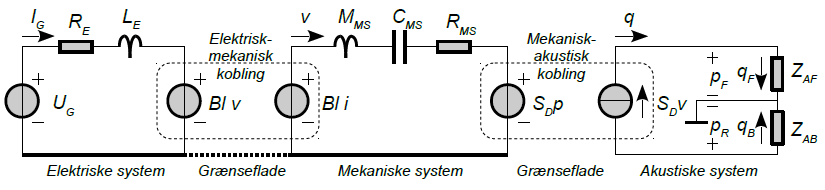
\includegraphics[width=\linewidth]{graphics/30.png}
	\caption{Model af elektro-dynamiske højttaler. \href{http://www.torean.dk/artikel/Elektroakustik.pdf}{(Elektroakustik, TAS)}}
	\label{fig:30}
\end{figure}

\subsection{Snittegning}
\begin{itemize}
	\item Membranen kan kun bevæge sig i akseretningen (lodret). \item For en bashøjttaler kan	bagsidens lydtryk passere gennem huller i rammen og undertiden gennem et hul i magnetens	centerdel.
	\item For en diskanthøjttaler er bagsiden  spærret inde i et lukket rum.
\end{itemize}

\begin{figure} [H]
	\centering
	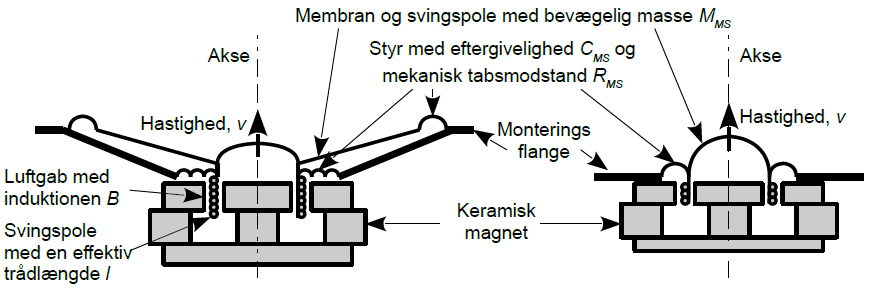
\includegraphics[width=\linewidth]{graphics/22.png}
	\caption{Snit igennem bashøjttaler (venstre) og diskant (højre).\\ \href{http://www.torean.dk/artikel/Elektroakustik.pdf}{(Elektroakustik, TAS)}}
	\label{fig:22}
\end{figure}

\begin{itemize}
	\item Bas
	\begin{itemize}
		\item Model gyldig til cirka \SI{500}{\hertz}
		\item Radius $a = \SI{100}{\milli\meter}$
	\end{itemize}
	\item Diskant
	\begin{itemize}
		\item Model gyldig til cirka \SI{2}{\kilo\hertz}
		\item Radius $a = \SI{12}{\milli\meter}$
	\end{itemize}
\end{itemize}

\subsection{Elektriske system}
\begin{itemize}
	\item Nær kobling mellem systemerne.
	\item Den elektriske impedans afspejler forholdene i det mekaniske- og akustiske system.
	\item Gør det er muligt at måle alle vigtige parametre for alle tre systemer alene fra den elektriske side.
\end{itemize}

\begin{figure} [H]
	\centering
	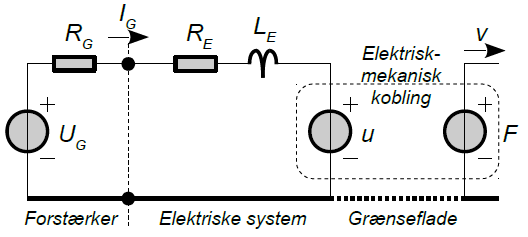
\includegraphics[width=0.8\linewidth]{graphics/23.png}
	\caption{Højttalerens elektriske system. \href{http://www.torean.dk/artikel/Elektroakustik.pdf}{(Elektroakustik, TAS)}}
	\label{fig:23}
\end{figure}
\begin{itemize}
	\item Højttalerens elektriske system består af følgende:
	\begin{itemize}
		\item Effektforstærkeren.
		\begin{itemize}
			\item Repræsenteret ved en spændingskilde $U_G$.
		\end{itemize}
		\item Modstanden $R_E$ fra svingspolens tråd.
		\item Selvinduktionen $L_E$ fra spolens	bevikling.
	\end{itemize} 
	\item Reaktionen fra det mekaniske system beskrives ved:
	\begin{itemize}
		\item Spændingskilden $Blv$ for Faradays induktionslov som følge af den hastighed $v$ svingspolen bevæger sig med.
	\end{itemize}
	\item Højttalerens "\textit{motor}" beskrives ved:	
	\begin{itemize}
		\item Kraftfaktoren $Bl$ hvor $B$ er magnetfeltets induktion og $l$ den effektive længde af tråd der befinder sig i magnetfeltet.
		\item Svingspolens selvinduktion er betydende over frekvensen $f_1$.
	\end{itemize}
\end{itemize}
    
\subsubsection{Typiske værdier}
\begin{itemize}
	\item $U_{G \,RMS}$ = \SI{2.83}{\volt} for \SI{1}{\watt} i nominelt \SI{8}{\ohm} svarer til $U_{G\, PEAK}$ = \SI{4}{\volt}.
	\item $R_E$ = DC modstand af ledningen (\si{\ohm}) typisk \SI{6.4}{\ohm} for \SI{8}{ohm} højtaler.
	\item $L_E$ = Selvinduktion af spolen (\si{\henry}) typisk \SI{1}{\milli\henry} for bas.
	\item $Bl$ = højttalerens kraftfaktor (\si{\tesla\meter}) typisk \SI{10}{\tesla\meter} (\SI{10}{\newton\per\ampere}).
\end{itemize}

\subsection{Mekaniske system}
\begin{itemize}
	\item Den elektrisk-mekanisk grænseflade beskrives ved højttalerens kraftfaktor $Bl$.
\end{itemize}

\begin{figure} [H]
	\centering
	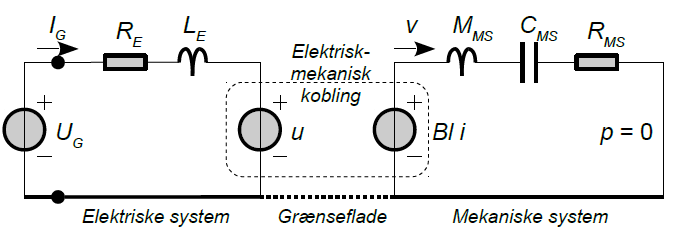
\includegraphics[width=0.95\linewidth]{graphics/24.png}
	\caption{Højttalerens elektro-mekaniske model. \href{http://www.torean.dk/artikel/Elektroakustik.pdf}{(Elektroakustik, TAS)}}
	\label{fig:24}
\end{figure}
\begin{itemize}
	\item Kraften på svingspolen er givet ved højttalerens kraftfaktor og strømmens styrke $F = Bl\, i$.
	\begin{itemize}
		\item Vil accelerere massen af svingspole og membran $M_{MS}$ efter Newtons anden lov. 
	\end{itemize} 	
	\item Styrene fungerer som en fjeder når svingspole og	membran bevæges.
	\begin{itemize}
		\item Trækker svingspole og membran tilbage igen i takt med at
		afstanden øges fra ligevægt.
	\end{itemize} 
	\item Intern friktion i styrene gør at der tabes energi og modelleres ved
	en mekanisk modstand $R_{MS}$. 
	\item Andre tabsmekanismer (dæmpningmsmaterialet i kabinettet og den afgivne lydeffekt) kan inkluderes ved at justere på $R_{MS}$.
\end{itemize}

\begin{figure} [H]
	\centering
	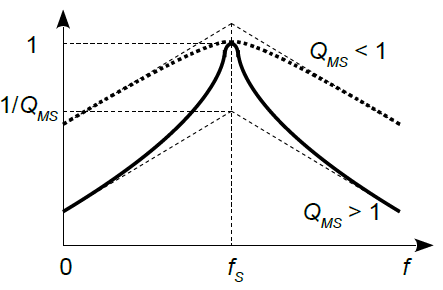
\includegraphics[width=0.6\linewidth]{graphics/26.png}
	\caption{Resonansfrekvensen vil dø ud. \href{http://www.torean.dk/artikel/Elektroakustik.pdf}{(Elektroakustik, TAS)}}
	\label{fig:26}
\end{figure}
\begin{itemize}
	\item Det mekaniske system vil svinge frivilligt hvis det sættes i gang.
	\item Hastigheden er proportional med frekvensen under den mekaniske resonans og den	aftager med frekvensen over resonansen.
	\item $Q_{MS}= \dfrac{1}{R_{MS}}\sqrt{\dfrac{M_{MS}}{C_{MS}}}$
\end{itemize}

\subsubsection{Typiske værdier}
\begin{itemize}
	\item $M_{MS}$ = Masse af bevægeligt system (\si{\kilogram}) typisk \SI{5}{\gram} ... \SI{20}{\gram}.
	\item $R_{MS}$ = Friktionstab (\si{\newton\second\per\meter}) typisk \SI{1}{\newton\second\per\meter}.
	\item $C_{MS}$ = Eftergivelighed af membranstyr (\si{\meter\per\newton}) typisk \SI{1}{\milli\meter\per\newton}.
	\item $f_S$ = Resonansfrekvens (\si{\hertz}) typisk \SI{35}{\hertz}.
	\item $Q_{MS}$ = Godhed af resonans typisk $0.35$.
\end{itemize}

\subsection{Akustiske system}
\begin{itemize}
	\item Den mekanisk-akustiske grænseflade udgøres af membranens areal $S_D$.
\end{itemize}

\begin{figure} [H]
	\centering
	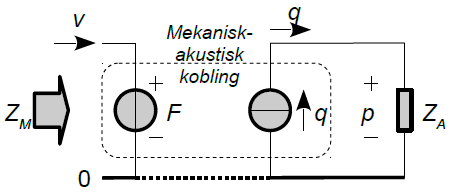
\includegraphics[width=0.65\linewidth]{graphics/25.png}
	\caption{Højttalerens makaniske-akustiske model \href{http://www.torean.dk/artikel/Elektroakustik.pdf}{(Elektroakustik, TAS)}}
	\label{fig:25}
\end{figure}


\subsubsection{Typiske værdier}
\begin{itemize}
	\item $S_D = \pi a^2$ = stemplets areal (\si{\square\meter})
	\item $q = S_Dv$ = volumehastighed (\si{\cubic\meter\per\second})
	\item $Z_A = \dfrac{p}{q}$ = strålingsimpedansen $\left(\dfrac{\si{\newton\meter^{-2}}}{\si{\cubic\meter\second^{-1}}}\right)$
\end{itemize}

\subsection{Thiele-Small parametre}
\begin{itemize}
	\item Højttalerens parametre beskrives i dens datablad som dens Thiele-Small parametre.
	\item Den elektro-mekaniske model kan benyttes til at bestemme værdien af højttalerens parametre.
\end{itemize}
\begin{figure} [H]
	\centering
	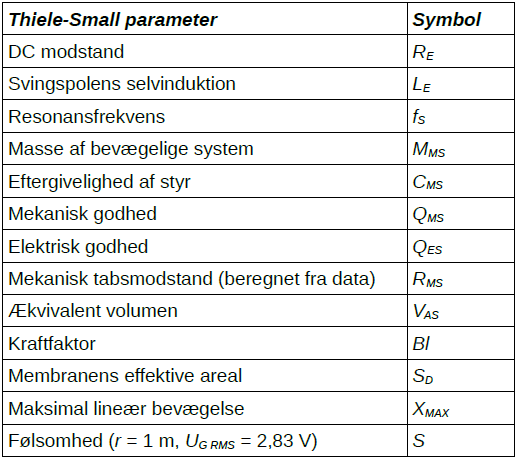
\includegraphics[width=0.85\linewidth]{graphics/27.png}
	\caption{Højttalerens makaniske-akustiske model \href{http://www.torean.dk/artikel/Elektroakustik.pdf}{(Elektroakustik, TAS)}}
	\label{fig:27}
\end{figure}

\subsection{Elektrisk og mekanisk impedans}
\begin{itemize}
	\item De seriekoblede impedanser fra det mekaniske system optræder nu som parallelkoblede reciprokke	impedanser i serie med svingspolens DC modstand og selvinduktion. 
	\item Impedansen vil have DC modstanden $R_E$ som mindste værdi. 
	\item Der vil være en top på $R_E + R_{ES}$ ved den frekvens $f_S$ hvor
	massen og eftergiveligheden går i resonans.
	\item Impedansen stiger for frekvenser over $f_1$ på grund af svingspolens selvinduktion. 
	\item Resonansfrekvens $f_S = \dfrac{1}{2\pi\sqrt{M_{MS}C_{MS}}}$
	\item Elektrisk impedans $Z_E = \dfrac{u}{i} = \dfrac{(Bl)^2}{Z_M}$
	\item Mekanisk impedans $Z_M = \dfrac{F}{v}= S_D^2Z_A$
	\item $F= S_D p$
\end{itemize}

\begin{figure} [H]
	\centering
	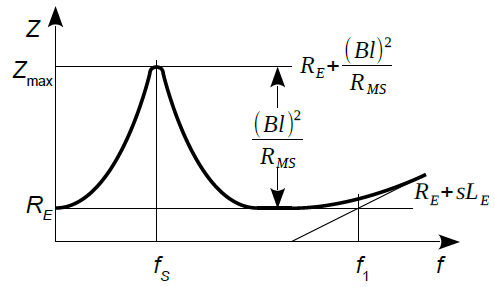
\includegraphics[width=0.7\linewidth]{graphics/28.png}
	\caption{Elektrisk og mekanisk impedans kurve \href{http://www.torean.dk/artikel/Elektroakustik.pdf}{(Elektroakustik, TAS)}}
	\label{fig:28}
\end{figure}

\subsection{Mekanisk og akustisk impedans}
\begin{itemize}
	\item Den akustisk impedans $Z_A$ er givet ved	forholdet mellem lydtryk og volumehastighed.
	\item Volumehastigheden $q$ der er hastigheden af det volumen af
	luft som membranen flytter.
	\item Lydtrykket $p$ der er den kraft luften påvirker membranen med som
	følge af bevægelsen.
	\item Strålingsimpedans $Z_A = \dfrac{p}{q} = \dfrac{Z_M}{S_D^2}$ 
	\item $q = S_D v$
\end{itemize}

\newpage\subsection{Lydtryk}
\begin{itemize}
	\item Højttalerens måleblad benytter et halvt rum.
	\item Højttaleren placeres med målemikrofonen i en afstand på \SI{1}{\meter} fra højttalerens akse.
	\item Effektforstærkeren indstilles til amplituden \SI{4}{\volt} for en effekt på \SI{1}{\watt} ved \SI{8}{\ohm}.
	\item Lydtrykket $p2\pi$ i afstanden $r$.
	\item $|p2\pi|=\dfrac{\rho S_D Bl}{2\pi r M_{MS}R_E}$ 
	\item $L = 20\log_{10}\left(\dfrac{p2\pi_{rms}}{p_{ref}}\right)$
\end{itemize}

\begin{figure} [H]
	\centering
	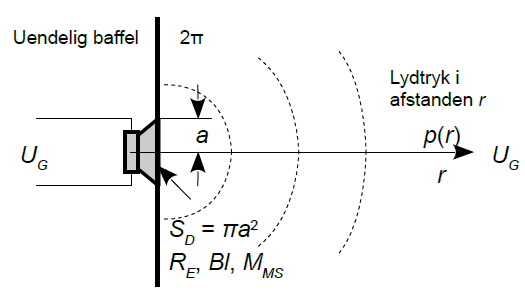
\includegraphics[width=0.7\linewidth]{graphics/29.png}
	\caption{Højttaleren bekrives ved placering i en uendeligt baffel ($2\pi$). \href{http://www.torean.dk/artikel/Elektroakustik.pdf}{(Elektroakustik, TAS)}}
	\label{fig:29}
\end{figure}

\subsubsection{Typiske værdier}
\begin{itemize}
	\item $p$ = amplituden af trykvariationen (\si{\pascal}) typisk \SI{1}{\pascal}.
	\item $r$ = afstanden til mikrofonen (\si{\meter}) typisk \SI{1}{\meter}.
\end{itemize}

\subsection{Øvelser}
\subsubsection{Øvelse 7.1}
Studer modellen med filnavnet: \mintinline{cpp}{PC Loudspeaker.xmcd}. Hvad betyder det at ændre styrets eftergivelighed ($C_{MS}$), det bevægelige systems masse ($M_{MS}$) og den elektriske dæmpning til det dobbelte af den nominelle værdi af $C_{MS}$, $M_{MS}$ og $R_E$. Fx én efter én? 
\newpage \noindent Det vi sigter efter er påvirkningen af resonansfrekvensen, dæmpningsfaktoren $Q$ (godheden) og lydtrykket i det frekvensuafhængige område.

\begin{figure} [H]
	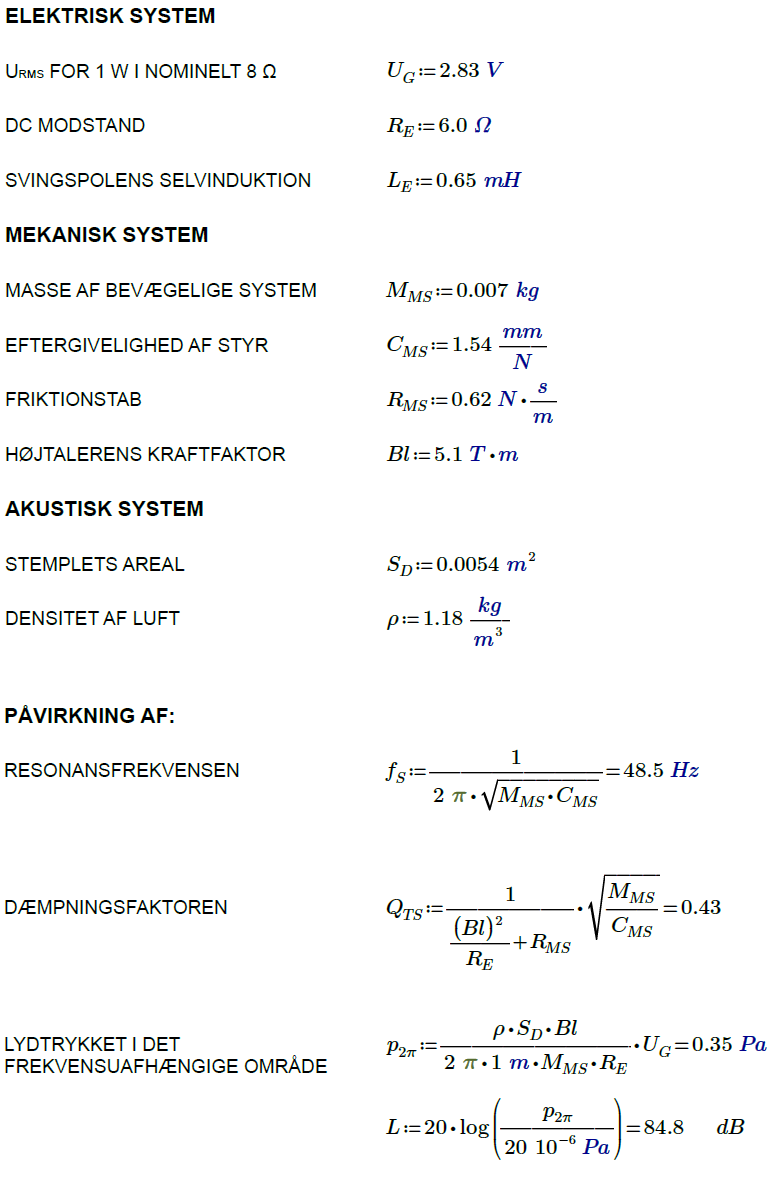
\includegraphics[width=\linewidth]{graphics/31.png}
\end{figure}

\newpage
\begin{itemize}
	\item Fordobling af den nominelle værdi af 
	\begin{itemize}
		\item $C_{MS}$
		\begin{itemize}
			\item Resonansfrekvensen $f_S$ falder til $\approx\SI{34}{\hertz}$
			\item Dæmpningfaktoren $Q$ ændres til $\approx 0.3$
		\end{itemize}
		\item $M_{MS}$
		\begin{itemize}
			\item Resonansfrekvensen $f_S$ falder til $\approx\SI{34}{\hertz}$
			\item Dæmpningfaktoren $Q$ ændres til $\approx 0.6$
			\item Lydtrykket $L$ falder til $\approx \SI{78}{\deci\bel}$
			\item Der skal mere energi til at systemet svinger
		\end{itemize} 
		\item $R_E$
		\begin{itemize}
			\item Resonansfrekvensen $f_S$ ændres ikke
			\item Dæmpningfaktoren $Q$ ændres til $\approx 0.8$
			\item Lydtrykket $L$ falder til $\approx \SI{79}{\deci\bel}$
			\item Der skal mere spænding til at levere samme strøm
		\end{itemize}
	\end{itemize}
\end{itemize}

\subsubsection{Øvelse 7.2}
Måling af lydtryk fra en højttaler (fx ved \SI{300}{\hertz}) og sammenligne med teorien for den massestyrede højttaler. Højttalerens mekaniske parametre ($S_D$, $Bl$, $M_{MS}$ og $R_E$) skal være kendt, mikrofonen skal være kalibreret og ligeledes for indstillingen af effektforstærkeren.

\subsubsection{Øvelse 7.3}
Måling af nogle af en højttalers parametre, som beskrevet i \href{http://www.torean.dk/artikel/Elektroakustik.pdf}{Elektroakustik,} side 33. For eksempel måling af DC modstand ($R_E$) med ohmmeter, stempelareal ($S_D$) med lineal og kraftfaktor ($Bl$) ved brug af en lille masse og strøm i svingspolen.
